\documentclass[tikz,border=2pt]{standalone}
\usepackage{amsmath,amssymb}
\usepackage{tikz}
\usetikzlibrary{arrows.meta,matrix}

\begin{document}
% Transposing swaps rows and columns: entry (i, j) moves to (j, i), a 2x3 matrix becomes 3x2.
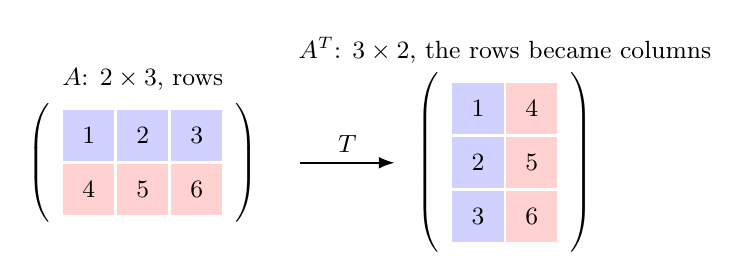
\begin{tikzpicture}[every node/.style={font=\small}, >={Latex[length=2mm]}]
	\matrix (A) [matrix of math nodes, nodes={minimum size=6.5mm, anchor=center}, left delimiter=(, right delimiter=), column sep=1pt, row sep=1pt] at (0,0) {
		|[fill=blue!18]| 1 & |[fill=blue!18]| 2 & |[fill=blue!18]| 3 \\
		|[fill=red!18]| 4 & |[fill=red!18]| 5 & |[fill=red!18]| 6 \\
	};
	\node[anchor=south, font=\small] at (A.north) {$A$: $2\times3$, rows};
	\draw[->, thick] (2.0,0) -- (3.2,0) node[midway, above] {$T$};
	\matrix (B) [matrix of math nodes, nodes={minimum size=6.5mm, anchor=center}, left delimiter=(, right delimiter=), column sep=1pt, row sep=1pt] at (4.6,0) {
		|[fill=blue!18]| 1 & |[fill=red!18]| 4 \\
		|[fill=blue!18]| 2 & |[fill=red!18]| 5 \\
		|[fill=blue!18]| 3 & |[fill=red!18]| 6 \\
	};
	\node[anchor=south, font=\small] at (B.north) {$A^{T}$: $3\times2$, the rows became columns};
\end{tikzpicture}
\end{document}
